% document formatting 
\documentclass[10pt]{article}
\usepackage[utf8]{inputenc}
\usepackage[left=1in,right=1in,top=1in,bottom=1in]{geometry}
\usepackage[T1]{fontenc}
\usepackage{xcolor}

% math symbols, etc.
\usepackage{amsmath, amsfonts, amssymb, amsthm}
\usepackage{dsfont}

% lists
\usepackage{enumerate}

% images
\usepackage{graphicx} % for images
\usepackage{tikz}

% code blocks
\usepackage{minted, listings} 

% verbatim greek
\usepackage{alphabeta}
\DeclareMathOperator*{\argmin}{arg\,min}
\DeclareMathOperator*{\argmax}{arg\,max}
\newcommand{\dd}{\text{d}}

\graphicspath{{./assets/images/}}

\title{02-620 Week 7 \\ \large{Machine Learning for Scientists}}
 
\author{Aidan Jan}

\date{\today}

\begin{document}
\maketitle
\section*{Probabilistic Graphical Models}
Essentially, a probability distribution, plus a graph.  \textbf{Probabilistic graphical models} define joint probability distributions
\begin{center} 
	\includegraphics*[width=\textwidth]{W7_1.png} 
\end{center}
\begin{itemize}
	\item Nodes represent \textbf{random variables}
	\item Edges represent \textbf{probabilistic dependencies}
\end{itemize}

\subsection*{Intuition of Probabilistic Graphical Models}
\begin{itemize}
	\item Key idea:
	\begin{itemize}
	    \item Conditional independence assumptions are useful
	    \begin{itemize}
	        \item For example, Naive Bayes: $P(X_1, \dots X_J | Y) = \prod_{i = 1}^J P(X_i | Y)$
        \end{itemize}
	    \item Sets of conditional independence assumptions are expressed via graph structure
    \end{itemize}
\end{itemize}

\subsubsection*{Examples}
Probabilistic graphical models model distribution of factors in causal interference.
\begin{center} 
	\includegraphics*[width=0.5\textwidth]{W7_2.png} 
\end{center}
\[P(S, Y, L) = P(Y | S) P(L | S) P(S) \rightarrow Y \perp L | S\]

Probabilistic graphical models model distribution in gene regulatory networks
\begin{itemize}
	\item Probability distribution and graph
	\item Breast cancer, estrogen receptor pathway
\end{itemize}
\begin{center} 
	\includegraphics*[width=0.7\textwidth]{W7_3.png} 
\end{center}
\[P(NCAPG, FOS, \cdots) = P(NCAPG) P(FOS | NCAPG) \cdots\]

\subsection*{Model Overview}
\begin{itemize}
	\item \textbf{Model}: directed acyclic graph (DAG), Bayesian network (BN)
	\item \textbf{Inference}: inferring hidden information from the model
	\item \textbf{Learning}:
	\begin{itemize}
	    \item Learning the probability distribution with known graph
	    \item Jointly learning the probability distribution and graph
    \end{itemize}
\end{itemize}

\subsubsection*{Example}
Events in an alarm system
\begin{center}
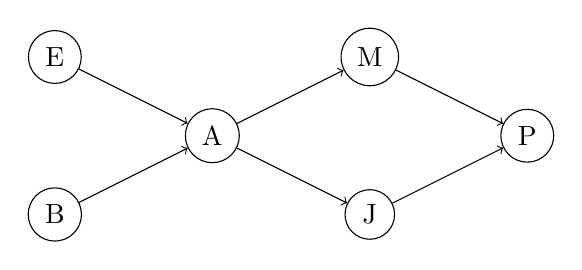
\begin{tikzpicture}
    \node[draw, circle] at (0, 0) (B) {B};
    \node[draw, circle] at (0, 2) (E) {E};
    \node[draw, circle] at (2, 1) (A) {A};
    \node[draw, circle] at (4, 0) (J) {J};
    \node[draw, circle] at (4, 2) (M) {M};
    \node[draw, circle] at (6, 1) (P) {P};

    \draw[->] (B) -- (A);
    \draw[->] (E) -- (A);
    \draw[->] (A) -- (J);
    \draw[->] (A) -- (M);
    \draw[->] (J) -- (P);
    \draw[->] (M) -- (P);
\end{tikzpicture}
\end{center}
\begin{itemize}
	\item $B$ - Burglary occurs
	\item $E$ - Earthquake occurs
	\item $A$ - Alarm goes off
	\item $J$ - John calls police
	\item $M$ - Mary calls police
	\item $P$ - Police comes
\end{itemize}

\subsubsection*{DAGs as dependency}
A directed acyclic graph (DAG) defines dependency between variables.  (A DAG is defined by a set of nodes and a set of directed edges.)
\begin{itemize}
	\item A DAG cannot have cycles!
\end{itemize}
Terminology:
\begin{itemize}
	\item Parents of node $A$: $B$, $E$
	\item Children of node $A$: $J$, $M$
	\item Descendants of node $A$: $J$, $M$, $P$
\end{itemize}

\subsubsection*{Bayesian network defines joint distribution}
\begin{itemize}
	\item Nodes are random variables
	\item Edges are probabilistic dependencies
	\item Each node is associated with a \textbf{conditional probability distribution given its parents}
	\begin{itemize}
	    \item $P(X_i | Pa(X_i))$ for each $X_i$
	    \item $Pa(X)$ = immediate parents of $X$ in the graph.
    \end{itemize}
\end{itemize}
\begin{center}
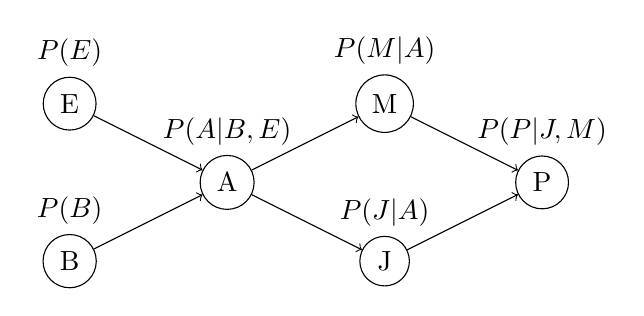
\begin{tikzpicture}
    \node[draw, circle, label=above:{$P(B)$}] at (0, 0) (B) {B};
    \node[draw, circle, label=above:{$P(E)$}] at (0, 2) (E) {E};
    \node[draw, circle, label=above:{$P(A | B, E)$}] at (2, 1) (A) {A};
    \node[draw, circle, label=above:{$P(J | A)$}] at (4, 0) (J) {J};
    \node[draw, circle, label=above:{$P(M | A)$}] at (4, 2) (M) {M};
    \node[draw, circle, label=above:{$P(P | J, M)$}] at (6, 1) (P) {P};

    \draw[->] (B) -- (A);
    \draw[->] (E) -- (A);
    \draw[->] (A) -- (J);
    \draw[->] (A) -- (M);
    \draw[->] (J) -- (P);
    \draw[->] (M) -- (P);
\end{tikzpicture}
\end{center}
A general bayesian network \textbf{joint distribution} over random variables $X_1, \cdots, X_n$ is given by
\[P(X_1, \dots, X_n) = \prod_i P(X_i | Pa(X_i))\]
In our example, we have
\[P(B, E, A, J, M, P) = P(B) P(E) P(A | B, E) P(J | A) P(M | A) P(P | J, M)\]
Why can't we have cycles?
\begin{itemize}
	\item What would happen to the probabilities if we have a cycle?
	\item Probabilities would be dependent on each other in a cycle, which does not make sense.
\end{itemize}

\subsection*{Summary: Constructing a Bayesian Network}
\begin{enumerate}
	\item Identify the random variables
	\item Determine the graph (the conditional dependencies)
	\item Determine the conditional probability distribution
\end{enumerate}

\subsection*{Factoring Joint Distributions}
\begin{itemize}
	\item Consider 5 binary random variabbles: $M, J, A, B, E$
	\item Chain rule for \textbf{general} factorization (no structure assumed:)
	\begin{align*}
        P(M, J, A, B, E) &= P(M | J, A, B, E) P(J, A, B, E) \\
        &= P(M | J, A, B, E) P(J | A, B, E) P(A, B, E) \\
        &= P(M | J, A, B, E) P(J | A, B, E) P(A | B, E) P(B, E) \\
        &= P(M | J, A, B, E) P(J | A, B, E) P(A | B, E) P(B | E) P(E) \\
    \end{align*}
    \item What is the directed acyclic graph (DAG) that corresponds to this factorization?
\end{itemize}
\[P(M | J, A, B, E) \textcolor{red}{P(J | A, B, E)} \textcolor{orange}{P(A | B, E)} \textcolor{green}{P(B | E)} \textcolor{blue}{P(E)}\]
\begin{center} 
	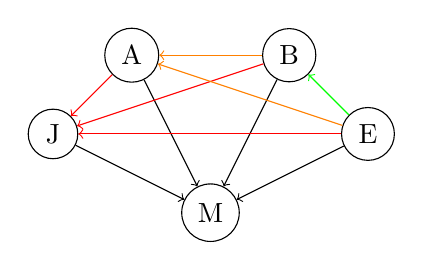
\begin{tikzpicture}
        \node[draw, circle] at (0, 0) (M) {M};
        \node[draw, circle] at (-2, 1) (J) {J};
        \node[draw, circle] at (-1, 2) (A) {A};
        \node[draw, circle] at (1, 2) (B) {B};
        \node[draw, circle] at (2, 1) (E) {E};

        \draw[->] (J) -- (M);
        \draw[->] (A) -- (M);
        \draw[->] (B) -- (M);
        \draw[->] (E) -- (M);
        
        \draw[->, red] (A) -- (J);
        \draw[->, red] (B) -- (J);
        \draw[->, red] (E) -- (J);

        \draw[->, orange] (B) -- (A);
        \draw[->, orange] (E) -- (A);
        
        \draw[->, green] (E) -- (B);
    \end{tikzpicture}
\end{center}

Number of parameters for general factorization:
\begin{itemize}
	\item $P(E) = 1$ ($E$ is the only parameter)
    \item $P(B | E) = 2$ ($E$ can either by 0 or 1, so we need $P(B | E = 0)$ and $P(B | E = 1)$, 2 parameters)
    \item $P(A | B, E) = 4$ ($B$ and $E$ have 4 combinations)
    \item $P(J | A, B, E) = 8$ (etc.)
    \item $P(M | J, A, B, E) = 16$
    \item Total: 31. 
\end{itemize}
The number of parameters is exponential! 
\begin{itemize}
	\item Better approach: Let's use our domain knowledge!
\end{itemize}
Earlier, we determined that $P(M, J, A, B, E) = P(B) P(E) P(A | B, E) P(J | A) P(M | A)$
\begin{itemize}
	\item $P(B) = 1$
	\item $P(E) = 1$
	\item $P(A | B, E) = 4$
	\item $P(J | A) = 2$
	\item $P(M | A) = 2$
	\item Total: 10.
	\item We saved 21 parameters!
\end{itemize}

\subsection*{Summary}
Directed acyclic graphs (DAG):
\begin{itemize}
	\item Nodes and directed edges
	\item No cycles
\end{itemize}
Bayesian networks:
\begin{itemize}
	\item Joint distribution
    \[P(X_1, \dots, X_n) = \prod_i P(X_i | Pa(X_i))\]
    \item $Pa(X)$ = immediate parents of $X$ in the graph.
    \item More intuitive representation, fewer parameters
\end{itemize}

\subsection*{Inference with Graphical Models}
Inference on graph:
\begin{itemize}
	\item Markov blanket
	\item d-separation
\end{itemize}
Inference on probability distribution
\begin{itemize}
	\item Enumeration
	\item Variable elimination
	\item Stochastic inference
\end{itemize}

\subsection*{Conditional Independence}
Given a Bayesian network, one can answer questions about \textbf{conditional independence} of two variabes given other variables, simply by \textbf{examining the graph structure}.
\begin{itemize}
	\item \textbf{Markov blanket:} conditional independence between one variable and the rest of the variables
	\[B \perp J, M | A, E\]
	\item \textbf{D-separation:} conditional independence between two variables
	\[B \perp J | A\]
\end{itemize}
How to check independence?
\begin{itemize}
	\item $A$ and $B$ are independent if and only if $P(A, B) = P(A) P(B)$
	\item Alternatively, $A$ and $B$ are independent if and only if $P(A | B) = P(A)$
	\item Similarly, $A$ and $B$ are independent given $C$ if and only if
	\begin{itemize}
	    \item $P(A, B|C) = P(A | C) P(B | C)$ or
	    \item $P(A | B, C) = P(A | C)$
    \end{itemize}
\end{itemize}

\subsection*{Bayesian Networks}
\subsubsection*{Markov Chain Example:}
Markov chains make the assumption that the future only depends on the present. (e.g., only the state we are currently on).  We can therefore model a Markov Chain as a Bayesian network like the following:
\begin{center}
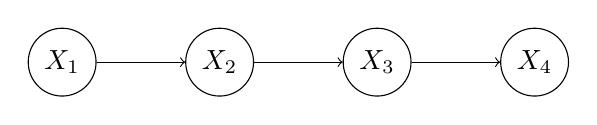
\begin{tikzpicture}
    \node[draw, circle] at (0, 0) (0) {$X_1$};
    \node[draw, circle] at (2, 0) (1) {$X_2$};
    \node[draw, circle] at (4, 0) (2) {$X_3$};
    \node[draw, circle] at (6, 0) (3) {$X_4$};

    \draw[->] (0) -- (1);
    \draw[->] (1) -- (2);
    \draw[->] (2) -- (3);
\end{tikzpicture}
\end{center}
\begin{itemize}
	\item Factorization: 
	\[P(X_1, X_2, X_3, X_4) = P(X_1) P(X_2 | X_1) P(X_3 | X_2) P(X_4 | X_3)\]
	\item Is $X_2$ independent of $X_4$?  
    \begin{itemize}
	    \item No.  $P(X_4 | X_2) \neq P(X_4)$.  If we are currently at $X_2$ in time, then $X_4$ definitely depends on the outcome of $X_2$ since it is in the future.
    \end{itemize}
	\item Is $X_2$ independent of $X_4$ given $X_3$? 
	\begin{itemize}
	    \item Yes.  $P(X_4 | X_2, X_3) = P(X_4 | X_3)$.  If we are given $X_3$, we have the outcome already, so the past ($X_2$) does not matter.
    \end{itemize}
	\item Are $X_1$ and $X_4$ independent given $X_2$?  
	\begin{itemize}
	    \item Yes.  $P(X_4 | X_2, X_1) = P(X_4 | X_2)$.  If we know the outcome of $X_2$, then $X_1$ is part of the past.
    \end{itemize}
\end{itemize}

\subsection*{Markov Blankets}
Markov blankets define conditional independence between one random variable and the rest of the random variables.
\begin{center}
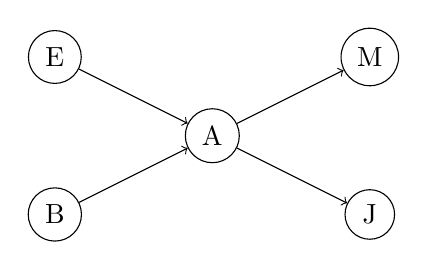
\begin{tikzpicture}
    \node[draw, circle] at (0, 0) (B) {B};
    \node[draw, circle] at (0, 2) (E) {E};
    \node[draw, circle] at (2, 1) (A) {A};
    \node[draw, circle] at (4, 0) (J) {J};
    \node[draw, circle] at (4, 2) (M) {M};

    \draw[->] (B) -- (A);
    \draw[->] (E) -- (A);
    \draw[->] (A) -- (J);
    \draw[->] (A) -- (M);
\end{tikzpicture}
\end{center}
\begin{itemize}
	\item Consider a node (e.g., $B$).  Let $S = \{E, A, J, M\}$ be the set of other nodes.
	\item Goal: find $S_1 \subset S$, such that
	\[B \perp S \setminus S_1 | S_1\]
    \item In other words, $S_1$ contains all the information about $B$
    \item In a Bayesian network, \textbf{a variable is conditionally independent of all other variables} given its \textbf{(minimal) Markov blanket}
    \begin{itemize}
	    \item The (minimal) Markov blanket of a node is all of its parents, children, and co-parents of children.
    \end{itemize}
\end{itemize}
In this example:
\begin{itemize}
	\item Markov blanket for $B$ is $P(B | E, A, J, M) = P(B | E, A)$
	\item Markov blanket for $A$ is everything.
	\item Markov blanket for $J$ is $P(J | E, A, B, M) = P(J | A)$
\end{itemize}

\subsection*{d-separation}
d-separation defines conditional independence between two random variables
\begin{itemize}
	\item Question: Are $X$ and $Y$ conditionally independent given evidence variables in $\{Z\}$?
	\[??? U \perp V | \{W, X, Y\}\]
    \item Yes, if $X$ and $Y$ are ``d-separated'' by $\{Z\}$
    \begin{itemize}
	    \item Consider all (undirected) paths from $X$ to $Y$
	    \item All paths inactive = independence
    \end{itemize}
\end{itemize}
\begin{center}
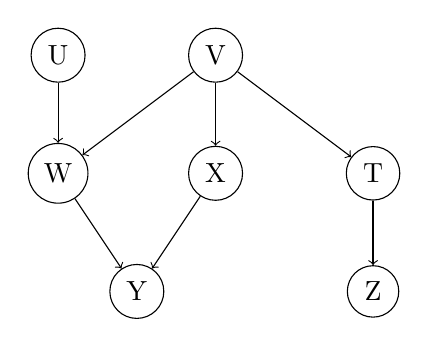
\begin{tikzpicture}
    \node[draw, circle] at (0, 0) (U) {U};
    \node[draw, circle] at (2, 0) (V) {V};
    \node[draw, circle] at (0, -1.5) (W) {W};
    \node[draw, circle] at (2, -1.5) (X) {X};
    \node[draw, circle] at (4, -1.5) (T) {T};
    \node[draw, circle] at (1, -3) (Y) {Y};
    \node[draw, circle] at (4, -3) (Z) {Z};

    \draw[->] (U) -- (W);
    \draw[->] (V) -- (W);
    \draw[->] (V) -- (X);
    \draw[->] (V) -- (T);
    \draw[->] (W) -- (Y);
    \draw[->] (X) -- (Y);
    \draw[->] (T) -- (Z);
\end{tikzpicture}
\end{center}

\subsection*{d-separation: Inactive paths}
A path is \textbf{inactive} if there is an inactive triple on the path:
\begin{itemize}
	\item Causal chain $X \rightarrow B \rightarrow Y$, where $B \in \{Z\}$
	\item Common cause $X \leftarrow B \rightarrow Y$, where $B \in \{Z\}$
	\item Common effect (aka v-structure) $X \rightarrow B \leftarrow Y$ where $B$ and its descendants not in $\{Z\}$
\end{itemize}
One inactive triple means the path is blocked or inactive.
\begin{center}
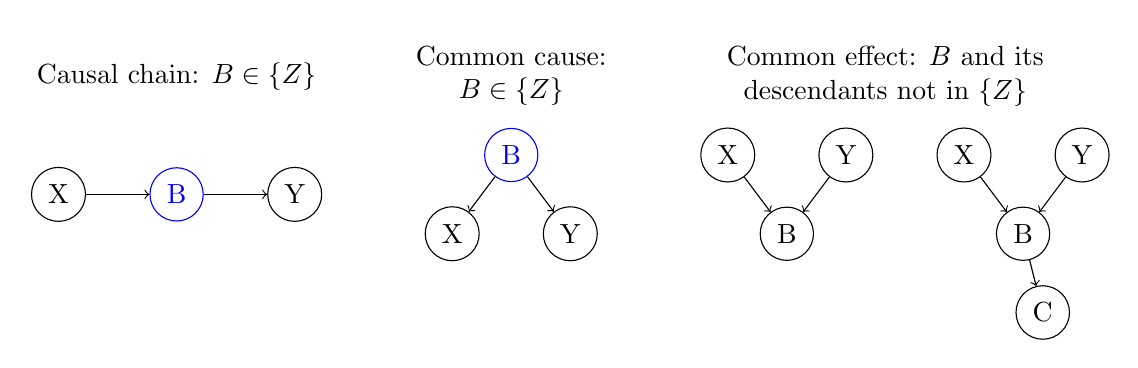
\begin{tikzpicture}
    \node[draw, circle] at (0, 0) (1X) {X};
    \node[draw, circle, blue] at (1.5, 0) (1B) {B};
    \node[draw, circle] at (3, 0) (1Y) {Y};

    \node[draw, circle] at (5, -0.5) (2X) {X};
    \node[draw, circle, blue] at (5.75, 0.5) (2B) {B};
    \node[draw, circle] at (6.5, -0.5) (2Y) {Y};

    \node[draw, circle] at (8.5, 0.5) (3X) {X};
    \node[draw, circle] at (9.25, -0.5) (3B) {B};
    \node[draw, circle] at (10, 0.5) (3Y) {Y};
    \node[draw, circle] at (11.5, 0.5) (4X) {X};
    \node[draw, circle] at (12.25, -0.5) (4B) {B};
    \node[draw, circle] at (13, 0.5) (4Y) {Y};
    \node[draw, circle] at (12.5, -1.5) (4C) {C};

    \draw[->] (1X) -- (1B);
    \draw[->] (1B) -- (1Y);

    \draw[->] (2B) -- (2X);
    \draw[->] (2B) -- (2Y);

    \draw[->] (3X) -- (3B);
    \draw[->] (3Y) -- (3B);

    \draw[->] (4X) -- (4B);
    \draw[->] (4Y) -- (4B);
    \draw[->] (4B) -- (4C);

    \node[align=center] at (1.5, 1.5) {Causal chain: $B \in \{Z\}$};
    \node[align=center] at (5.75, 1.5) {Common cause: \\$B \in \{Z\}$};
    \node[align=center] at (10.5, 1.5) {Common effect: $B$ and its \\ descendants not in $\{Z\}$};

    \node at (0, 2) (placeholder) {};
\end{tikzpicture}
\end{center}

\subsection*{d-separation: algorithm}
\begin{itemize}
	\item Given query: if $X_i \perp X_j | \{X_{k_1}, \cdots, X_{k_n}\}$?
	\item List all (undirected) paths between $X_i$ and $X_j$
	\item Check if each path is inactive or blocked
	\item If all paths are inactive or blocked, then ``guaranteed that $X_i \perp X_j | \{X_{k_1}, \cdots, X_{k_n}\}$'' is true.
\end{itemize}

\subsection*{Examples}
\begin{center}
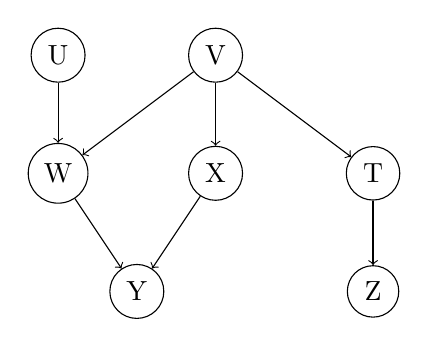
\begin{tikzpicture}
    \node[draw, circle] at (0, 0) (U) {U};
    \node[draw, circle] at (2, 0) (V) {V};
    \node[draw, circle] at (0, -1.5) (W) {W};
    \node[draw, circle] at (2, -1.5) (X) {X};
    \node[draw, circle] at (4, -1.5) (T) {T};
    \node[draw, circle] at (1, -3) (Y) {Y};
    \node[draw, circle] at (4, -3) (Z) {Z};

    \draw[->] (U) -- (W);
    \draw[->] (V) -- (W);
    \draw[->] (V) -- (X);
    \draw[->] (V) -- (T);
    \draw[->] (W) -- (Y);
    \draw[->] (X) -- (Y);
    \draw[->] (T) -- (Z);
\end{tikzpicture}
\end{center}
\textbf{Example 1:}
\begin{itemize}
	\item Query: if $V \perp Z | \{\}$?
	\item Paths: 
	\begin{itemize}
	    \item V $\rightarrow$ T $\rightarrow$ Z:  Active (causal chain)
    \end{itemize}
    \item Conclusion: independence not guaranteed
\end{itemize}
\textbf{Example 2:}
\begin{itemize}
	\item Query: if $V \perp Z | \{T\}$?
	\item Paths: 
	\begin{itemize}
	    \item V $\rightarrow$ T $\rightarrow$ Z:  Inactive (causal chain $T$ observed)
    \end{itemize}
    \item Conclusion: independence guaranteed
\end{itemize}
\textbf{Example 3:}
\begin{itemize}
	\item Query: if $U \perp V | \{\}$?
	\item Paths: 
	\begin{itemize}
	    \item U $\rightarrow$ W $\rightarrow$ V:  Inactive (common effect, $W$ and descendants unobserved)
	    \item U $\rightarrow$ W $\rightarrow$ Y $\rightarrow$ X $\rightarrow$ V:  Inactive
	    \begin{itemize}
	        \item U $\rightarrow$ W $\rightarrow$ Y: active (causal chain)
	        \item W $\rightarrow$ Y $\rightarrow$ X: inactive (common effect)
	        \item Y $\rightarrow$ X $\rightarrow$ V: active (causal chain)
        \end{itemize}
    \end{itemize}
    \item Conclusion: independence guaranteed
\end{itemize}
\textbf{Example 4:}
\begin{itemize}
	\item Query: if $U \perp V | \{W\}$?
	\item Paths: 
	\begin{itemize}
	    \item U $\rightarrow$ W $\rightarrow$ V:  Active (common effect, $W$ observed)
	    \item U $\rightarrow$ W $\rightarrow$ Y $\rightarrow$ X $\rightarrow$ V:  Don't care
    \end{itemize}
    \item Conclusion: independence not guaranteed
\end{itemize}
\textbf{Example 5:}
\begin{itemize}
	\item Query: if $U \perp V | \{X\}$?
	\item Paths: 
	\begin{itemize}
	    \item U $\rightarrow$ W $\rightarrow$ V:  Inactive (common effect, $W$ and descendants unobserved)
	    \item U $\rightarrow$ W $\rightarrow$ Y $\rightarrow$ X $\rightarrow$ V:  Inactive
	    \begin{itemize}
	        \item U $\rightarrow$ W $\rightarrow$ Y: active (causal chain)
	        \item W $\rightarrow$ Y $\rightarrow$ X: inactive (common effect)
	        \item Y $\rightarrow$ X $\rightarrow$ V: inactive (causal chain)
        \end{itemize}
    \end{itemize}
    \item Conclusion: independence guaranteed
\end{itemize}
\textbf{Example 6:}
\begin{itemize}
	\item Query: if $U \perp V | \{Y\}$?
	\item Paths: 
	\begin{itemize}
	    \item U $\rightarrow$ W $\rightarrow$ V:  Active (common effect, descendant $Y$ observed)
	    \item U $\rightarrow$ W $\rightarrow$ Y $\rightarrow$ X $\rightarrow$ V:  Active
	    \begin{itemize}
	        \item U $\rightarrow$ W $\rightarrow$ Y: active (causal chain)
	        \item W $\rightarrow$ Y $\rightarrow$ X: active (common effect, $Y$ observed)
	        \item Y $\rightarrow$ X $\rightarrow$ V: active (causal chain)
        \end{itemize}
    \end{itemize}
    \item Conclusion: independence not guaranteed
\end{itemize}
\textbf{Example 7:}
\begin{itemize}
	\item Query: if $U \perp V | \{Z\}$?
	\item Paths: 
	\begin{itemize}
	    \item U $\rightarrow$ W $\rightarrow$ V:  Inactive (common effect, $W$ and descendants unobserved)
	    \item U $\rightarrow$ W $\rightarrow$ Y $\rightarrow$ X $\rightarrow$ V:  Inactive
	    \begin{itemize}
	        \item U $\rightarrow$ W $\rightarrow$ Y: active (causal chain)
	        \item W $\rightarrow$ Y $\rightarrow$ X: inactive (common effect, $Y$ unobserved)
	        \item Y $\rightarrow$ X $\rightarrow$ V: active (causal chain)
        \end{itemize}
    \end{itemize}
    \item Conclusion: independence guaranteed
\end{itemize}
\textbf{Example 8:}
\begin{itemize}
	\item Query: if $W \perp X | \{\}$?
	\item Paths: 
	\begin{itemize}
	    \item W $\rightarrow$ V $\rightarrow$ X:  Active (common effect, $V$ unobserved)
	    \item U $\rightarrow$ W $\rightarrow$ Y $\rightarrow$ X $\rightarrow$ V:  Don't care
    \end{itemize}
    \item Conclusion: independence not guaranteed
\end{itemize}
\textbf{Example 9:}
\begin{itemize}
	\item Query: if $X \perp T | \{V\}$?
	\item Paths: 
	\begin{itemize}
	    \item X $\rightarrow$ V $\rightarrow$ T:  Inactive (common cause, $V$ observed)
	    \item X $\rightarrow$ Y $\rightarrow$ W $\rightarrow$ V $\rightarrow$ T:  Inactive
	    \begin{itemize}
	        \item X $\rightarrow$ Y $\rightarrow$ W: inactive (common effect)
	        \item Y $\rightarrow$ W $\rightarrow$ V: active (causal chain)
	        \item W $\rightarrow$ V $\rightarrow$ T: inactive (common cause)
        \end{itemize}
    \end{itemize}
    \item Conclusion: independence guaranteed
\end{itemize}
\textbf{Example 10:}
\begin{itemize}
	\item Query: if $X \perp W | \{U\}$?
	\item Paths: 
	\begin{itemize}
	    \item W $\rightarrow$ V $\rightarrow$ X:  Active (common effect, $V$ unobserved)
	    \item W $\rightarrow$ Y $\rightarrow$ X: Don't care
    \end{itemize}
    \item Conclusion: independence not guaranteed
\end{itemize}

\subsection*{Summary}
Markov blanket
\begin{itemize}
	\item In a Bayesian network, a variable is conditionally independent of all other variables given its (minimal) Markov blanket
	\item A (minimal) Markov blanket of a node is all of its parents, children, and co-parents of children
\end{itemize}
D-separation
\begin{itemize}
	\item Question: Are $X$ and $Y$ conditionally independent given evidence vars in $\{Z\}$?
	\item All paths inactive $\rightarrow$ independence
\end{itemize}
\end{document}